\chapter{實驗設計與結果}
\label{c:experiment}

在本章中,我們將在不同工作量下評估
以不同資料結構分別實作的持久化 LRU 的 (i) 速度 (ii) 記憶體用量。

\section{實驗環境}
實驗均在以下環境中進行

\begin{itemize}
\item CPU: AMD Ryzen 7 2700X (8 核心 16 執行緒、3.6 GHz、32K L1d 快取、64k L1i 快取、512K L2 快取、8M L3 快取)
\item 記憶體: DDR4 64 GB
\item 作業系統:Linux manjaro 4.19.36-1-MANJARO x86\_64
\item 編譯器: GCC 9.1.0
\end{itemize}

\section{資料結構}

我們以 C++ 17 撰寫了三種資料結構:

\begin{itemize}
\item 雜湊 + 雙向鏈表(3.4 節),每次以完全複製本身的方式來建立新版本
\item 持久化雜湊 + 持久化紅黑樹(3.4.1 節)
\item 持久化雜湊 + 持久化順序樹(3.4.2 節)
\end{itemize}

\section{速度}

\subsection{調整快取大小}

\begin{figure}[h!]
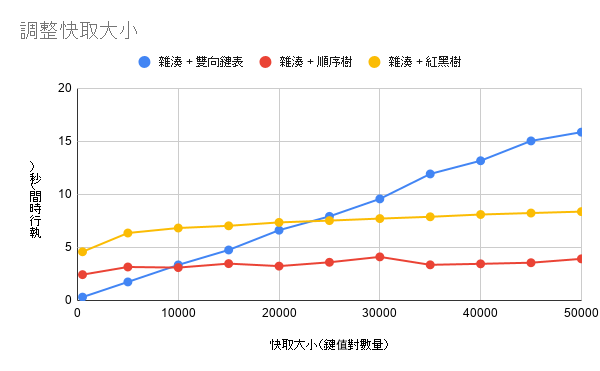
\includegraphics[width=\textwidth]{調整快取大小}
\caption{調整快取大小}
\end{figure}

\subsection{調整快取命中率}

\begin{figure}[h!]
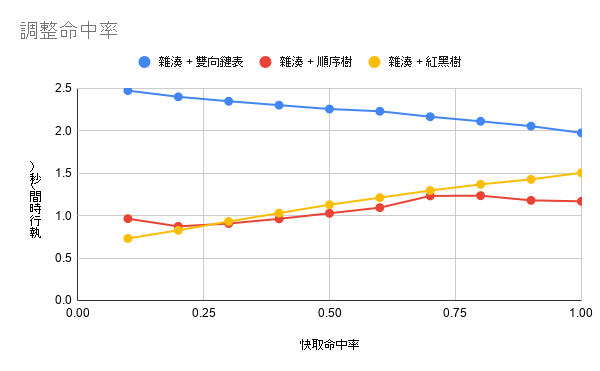
\includegraphics[width=\textwidth]{調整命中率}
\caption{調整命中率}
\end{figure}

\subsection{調整 put 比例}

調整 put 佔所有

\begin{figure}[h!]
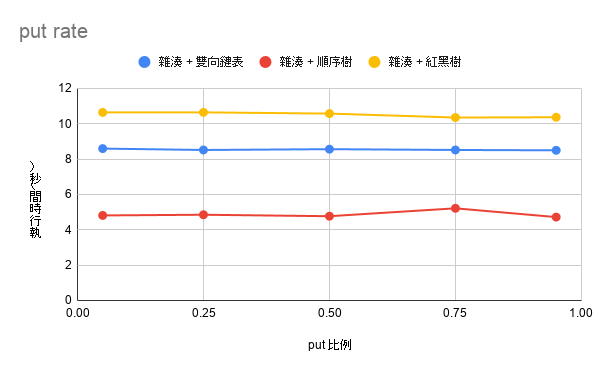
\includegraphics[width=\textwidth]{put_rate}
\caption{調整 put 比例}
\end{figure}

\subsection{記憶體用量}